\section{Solution Strategy}\label{solution-strategy}

\subsection{Conceptual Design}\label{conceptual-design}

Conceptually, the GPS\_Tracker framework consists of several abstract
components

\begin{longtable}[]{@{}ll@{}}
\caption{Conceptual Design components}\tabularnewline
\toprule
\begin{minipage}[b]{0.47\columnwidth}\raggedright
Component\strut
\end{minipage} & \begin{minipage}[b]{0.47\columnwidth}\raggedright
Description\strut
\end{minipage}\tabularnewline
\midrule
\endfirsthead
\toprule
\begin{minipage}[b]{0.47\columnwidth}\raggedright
Component\strut
\end{minipage} & \begin{minipage}[b]{0.47\columnwidth}\raggedright
Description\strut
\end{minipage}\tabularnewline
\midrule
\endhead
\begin{minipage}[t]{0.47\columnwidth}\raggedright
Analyzer\strut
\end{minipage} & \begin{minipage}[t]{0.47\columnwidth}\raggedright
An special entity that performs ETL operations on the data provided by
ClientApp.\strut
\end{minipage}\tabularnewline
\begin{minipage}[t]{0.47\columnwidth}\raggedright
ClientApp\strut
\end{minipage} & \begin{minipage}[t]{0.47\columnwidth}\raggedright
An entity installed on the user's phones that send information from the
sensors.\strut
\end{minipage}\tabularnewline
\begin{minipage}[t]{0.47\columnwidth}\raggedright
MessageBroker\strut
\end{minipage} & \begin{minipage}[t]{0.47\columnwidth}\raggedright
Protocol that the data from sensors is sent over.\strut
\end{minipage}\tabularnewline
\begin{minipage}[t]{0.47\columnwidth}\raggedright
DataBroker\strut
\end{minipage} & \begin{minipage}[t]{0.47\columnwidth}\raggedright
A sensor data receiver part. The terminating side of
MessageBroker.\strut
\end{minipage}\tabularnewline
\begin{minipage}[t]{0.47\columnwidth}\raggedright
DataBackend\strut
\end{minipage} & \begin{minipage}[t]{0.47\columnwidth}\raggedright
A component that provides data access methods for the end clients.\strut
\end{minipage}\tabularnewline
\begin{minipage}[t]{0.47\columnwidth}\raggedright
DataVisualizer\strut
\end{minipage} & \begin{minipage}[t]{0.47\columnwidth}\raggedright
An entity the user interacts with.\strut
\end{minipage}\tabularnewline
\begin{minipage}[t]{0.47\columnwidth}\raggedright
Storage\strut
\end{minipage} & \begin{minipage}[t]{0.47\columnwidth}\raggedright
A program that stores sensor data reliably and has a well-defined access
interface.\strut
\end{minipage}\tabularnewline
\bottomrule
\end{longtable}

\begin{figure}[H]
\centering
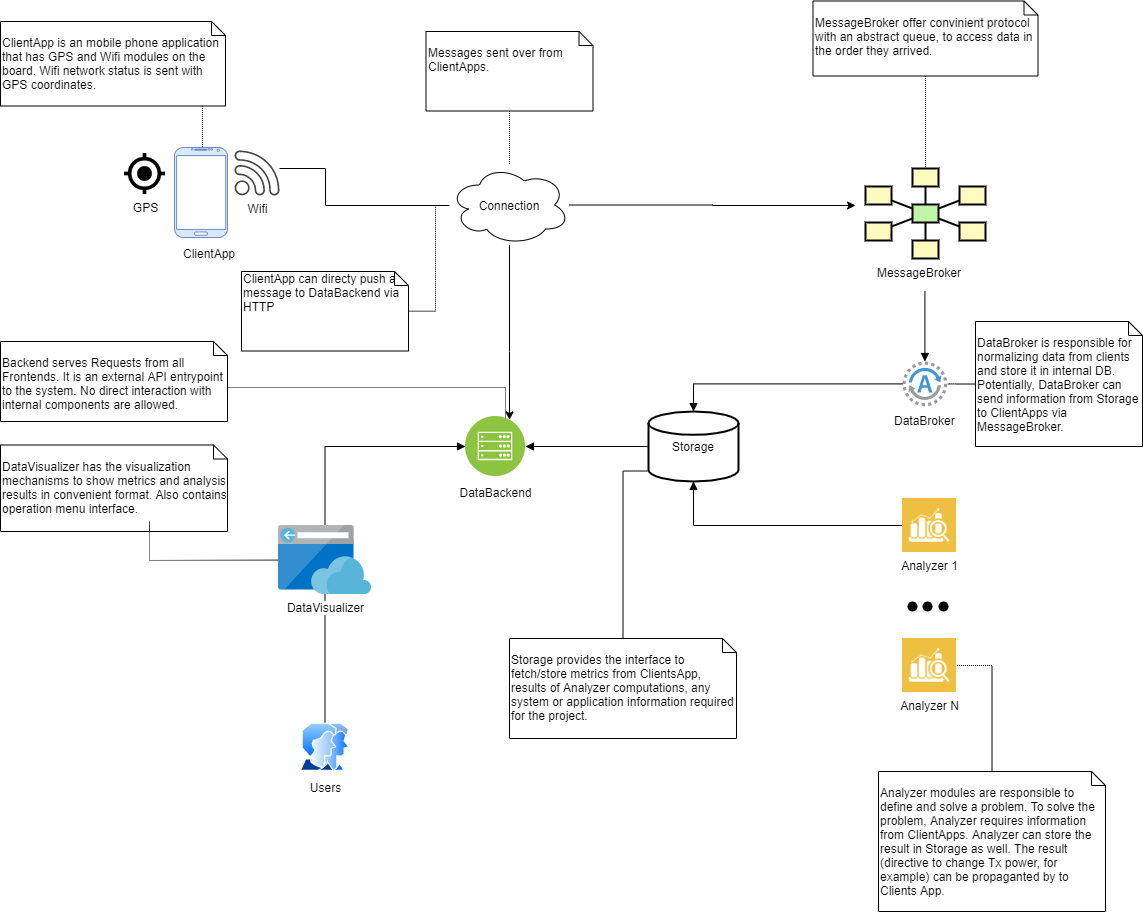
\includegraphics[width=\linewidth]{schemes/conceptual/ConceptualDiagram.png}
\caption{Conceptual Design Diagram}
\end{figure}


\subsection{Solution Approaches}\label{solution-approaches}

\subsubsection{Performance}\label{performance}

\paragraph{Goal}\label{goal}

The messages receiving an operation performing must be accomplished as
fast as possible.

\paragraph{Solution}\label{solution}

To accomplish that, a protocol with very low latency but still reliable
must be used. That must be a TCP/IP-based application protocol. There
are two possible choices:

\begin{itemize}
\tightlist
\item
  TCP-based protocols for a reliable connection, but may have higher
  latency.
\item
  UDP-based protocols for fast transmission without built-in reliable
  quality, but still has some of acknowledging mechanisms on the
  application level.
\end{itemize}

Moreover, all components must be aware of to be written with efficient
programming techniques and components.

\subsubsection{Reliability}\label{reliability}

\paragraph{Goal}\label{goal-1}

The communication sides must have a way to check if the message received
and interpreted correctly.

\paragraph{Solution}\label{solution-1}

For that, there must be checks in the end-to-end protocol, as well as
checks in the backend that received information stored.

\subsubsection{Scalability}\label{scalability}

\paragraph{Goal}\label{goal-2}

There must be an opportunity to easily increase the performance of the
framework if required.

\paragraph{Solution}\label{solution-2}

Publish/subscriber architecture pattern suits well the scalability
requirement. Each component can be changed separately by different
component regarding the proper interface implementation done.

\subsubsection{Usability}\label{usability}

\paragraph{Goal}\label{goal-3}

The human-to-machine communication must have a user-friendly interface.
There should be no problem with using the framework.

\paragraph{Solution}\label{solution-3}

For better understanding, a proper documentation section is available
for the user. The UI will be built using modern web technologies. That
would give good user-experience.

\subsubsection{Maintainability}\label{maintainability}

\paragraph{Goal}\label{goal-4}

Since the framework is quite complex, the additional complexity
definitely will harm possible production installation.

\paragraph{Solution}\label{solution-4}

To increase maintainability automation tools for development, deployment
and maintenance used. The framework configured to provide easy-to-use
instruments for the administrators.

To increase maintainability automation tools for development, deployment
and maintenance used. The framework configured to provide easy-to-use
instruments for the administrators.
